\chapter{Introduction}
\section{The high energy exploration}
According to \cite{} The triumph of the 20th century particle physics was the development of the Standard Model. Experiments determined the particle constituents of ordinary matter, and identified four forces binding matter and transforming it from one form to another. This success leads particle physicist to address even more fundamental questions, and explore deeper mysteries in science.\par
The Standard Model includes a third component beyond particles and forces, the Higgs mechanism. The Higgs mechanism permeates the universe, giving mass to the particles, and breaking the electro-weak force in two, the electromagnetic and the weak forces.\par
\begin{figure}[!hbt]
\centering
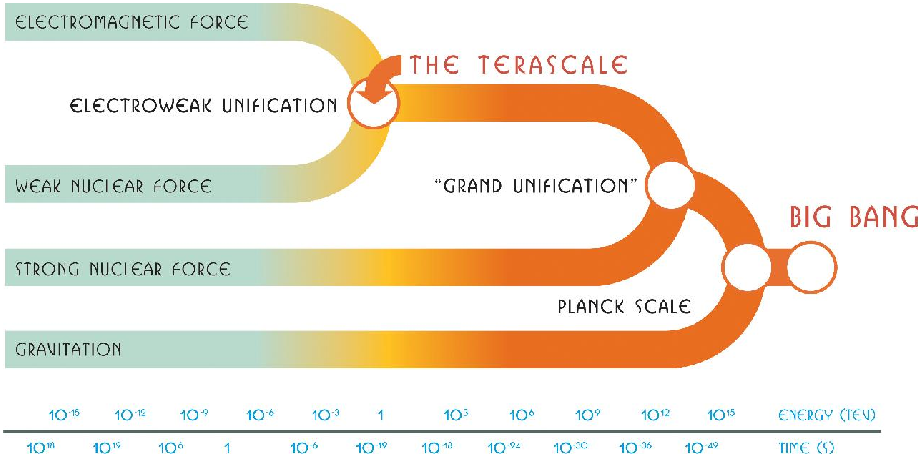
\includegraphics[scale=0.8,angle=0]{energyforce.pdf}\caption{The electromagnetic and electro-weak forces unify at the Terascale.}\label{f:energyforce}
\end{figure}
Experiments in the Terascale could test the idea that fundamental forces originate from a single unified force, see Fig. \ref{f:energyforce}, and search for evidence of a related unified origin of matter involving supersymmetry. They could distinguish among patterns of phenomena to judge different unification models, providing a telescopic view of the ultimate unification.\par
% \section*{The exploration of high energy physics}
% \addcontentsline{toc}{section}{The exploration of high energy physics}
There are two ways to explore the subatomic world, the first is to go to higher energy to discover new particles and measure their properties, the second is to increase the precision of the measurements to detect rare processes and make detailed studies.\par
The LHC allows the exploration of the electroweak symmetry breaking mechanism and other physical phenomena at the TeV scale, like the CP violation problem, the quark gluon plasma at the search of new physics beyond the Standard Model such as supersymmetry (SUSY) among others. The future linear collider beam energy will be determined by the LHC discoveries.\par
\textbf{Higgs searches:} The 4th of July of 2012, in a seminar held at CERN, the collaborations of the Experiments CMS and ATLAS presented an update of the Higgs of the Higgs searches status. At a confidence level of 4.9$\sigma$ for CMS \cite{TheCMSCollaboration21122012}, and 5.1$\sigma$ for ATLAS \cite{TheATLASCollaboration21122012} from the Higgsless Standard Model, signals of a boson with a mass around $m_h=125$~GeV were found with a strong spin-0 indication and coupling parameters consistent with the properties of the Standard Model Higgs Particle. First results on various rare production decay modes have been obtained but more data is needed to observe these models. Many analyses are ongoing and more updates are constantly presented.\par
\textbf{Heavy Flavour and CP Violation:} The experiments of the LHC, led by the LHCb, have carried out several important findings and measurements in the heavy flavour sector. New previously unobserved states have been observed for the very first time during the last years like the states $X_b$, $\Xi_a$ and $\Lambda_s^0$. Also the measurement of the quantum numbers of the states $X(3872)$ with $J^{PC}=1^{++}$, have been determined to the 8$\sigma$ level. The CP violation of the oscillation in D and B mesons have been measured to the 9.1$\sigma$ confidence level discovering the same violation in $B_s$ systems. The CP angle $\gamma$ is known with a precision without precedents ($\gamma=(67\pm12)$\textdegree). Finally, some very rare decays like $B_s\rightarrow\mu^+\mu^-$, $B^0\rightarrow K^*\mu^+\mu^-$ and $D_s^+\rightarrow\pi^+\mu^+\mu^-$ have been observed, with possible implications on the analysis of new physics.\par
\textbf{Quark-gluon Plasma:} The quark-gluon plasma is produced in ultra-relativistic heavy ion collisions. The conditions observed at the LHC experiments (ALICE, ATLAS and CMS) are in agreement with the observations carried out at RHIC. It has been confirmed that the hydrodynamics model helps in the understanding of the behaviour of the processes occurred during the collision. It is still far from being completely understood.\par
\textbf{SUSY and Dark Matter searches:} One of the problem that arises is the stabilization of the Higgs mass and its divergence when quantum divergence is considered. The solution involves a new principle of nature called supersymmetry (SUSY), a new symmetry that unifies bosons and fermions. After data collected during 2011 and 2012, SUSY searches at the LHC did not find any evidence of any light superpartner (squark or gluino) and it has pushed their mass limits beyond 1~TeV with the constrained model~\cite{Kraml:2012er}.\par
\vspace*{0.6cm}
The Second run of the LHC at 13~TeV will provide more information about the physics at high energies.\par

\subsection{Circular or linear colliders}
Higher energies have been usually explored with hadron colliders and the precision measurements has been done by lepton colliders, however, lepton circular colliders are limited by radiation. When particles traverse magnetic fields they emmit photons and this photons make the beam loose energy per turn given by
\begin{equation}
 \Delta E_{turn}=\frac{E^4}{3\rho m_0^4c^8}
\end{equation}
where $m_0$ is the rest mass of the particle, $c$ is the speed of light, $\rho$ is the curvature radius to the trajectory produced by the magnet and $E$ is the beam energy. The highest energy lepton collision, 209~GeV, have been reached with electron and positron coliding beams in LEP at CERN.  In spite of the 27~km circumference of LEP the beam energy was limited by synchrotron radiation losses, just compensated by a powerfull superconducting RF system providing up to 3640~MV per revolution \cite{Assmann:549223}.\par
% \section{Purpose of a linear collider}
\section{Purpose of a linear collider}
The physics potential of future linear colliders has been studied since the Standford Linear Collider (SLC)~\cite{Feldman88,SLC91}. The advantage of a linear lepton collider with respect to the LHC is the cleanliness of the events where two elementary particles with known kinematics and spin define the initial state. The resulting precision of the measurements is achievable because of the high resolution possible in the detector due to background processses well calculated and measured, a clean experimental environment, ability to scan systematically in c.o.m energy, possibility of high degree of polarization, and possibility for $\gamma\gamma$, $e^-e^-$, $e^-\gamma$ collisions.\par
\subsection{Physics in $e^+e^-$ colliders}
The confirmation of the Standard Model has been achieved through a combination of analyses from LEP, SLC, HERA, B-factories, Tevatron and the LHC and the gauge structure $SU(3)_C\times SU(2)_L\times U(1)_Y$. In this model the Higgs mechanism is responsible for the electroweak symmetry breaking and the masses of other particles.\par
A linear collider can be used to conclude if the boson found at LHC has the properties predicted by the Standard Model or if it is part of an extended Higgs sector as in~SUSY~\cites{Ellis:2008gj,Accomando:2004sz,Assmann:2000hg}. Figure~\ref{f:higgsch} shows the cross section of the Higgs bosson production mechanisms as a function of the c.o.m energy of the $e^+e^-$ collision.\par
One other aspect is that a linear collider can study the presence of composite structure of the Higgs particle and can measure precisely the electroweak coupling of the top quark by directly measuring the top quark mass.\par
A linear collider can also be used to explore the Kaluza-Klein theory of an extra-space dimension where gravitons propagate, and the deep study of couplings and spins in SUSY if there is signs of their existance in the LHC run 2.\par
\begin{figure}[h]
\centering
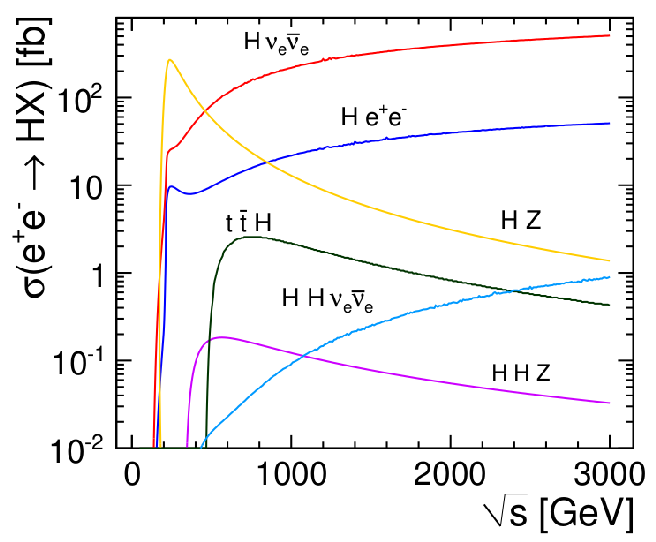
\includegraphics[scale=0.8,angle=0]{higgschannels.pdf}\caption{Cross section of Higgs production as a function of $\sqrt{s}$ for $m_h=120$~GeV.}\label{f:higgsch}
\end{figure}
 
\subsection{Rate of events}
Although cosmic rays could be of large energies, a large number of particle detections is required to obtain enough statistics to confirm the validity of a theory,  therefore the need of a collider.\par
Luminosity, $L$, is proportional to the number of collisions that are produced when two beams cross each other. The expression that relates luminosity, cross section $\sigma$ and the number of events produced $R$ is given by,
\begin{equation}
 R=L\sigma
\end{equation}
Luminosity will depend on the bunch population 	$n_b$ (assuming an equal number of particles for both beams) and their density distribution within the bunches.\par 
Linear colliders require to minimize the beam size at the Interaction Point (IP) of the two beams to recover the luminosity $L$ of a circular collider. Equation~(\ref{eq:lum}) highlights the dependence with beam size in the tranversal planes, where $f_{rep}$ is the repetion frequency of the two particle bunches collision, $E$ is the beam energy, and $\sigma_x$ and $\sigma_y$ are the horizontal and vertical beam sizes.
\begin{equation}
 L \propto \frac{f_{rep}n_b^2}{\sigma_x\sigma_y}\label{eq:lum}%\qquad\delta_{BS}\propto\frac{n_b^2E}{(\sigma_x+\sigma_y)^2}\label{eq:lum_rad}
\end{equation}
Table~\ref{t:lum_rad} shows how the beam size is decreased in the linear colliders SLC~\cite{PhysRevD.54.1}, CLIC~\cite{CLICdes} and ILC~\cite{ILCdes} (last two to be introduced in Section~\ref{s:lincoll}), to compensate lower repetition rate and charges when compared with the circular collider LEP \cite{Colliderparam}. Horizontal beam size is larger than vertical beam size in lepton colliders to preserve luminosity while mitigating the beam-beam effect called beam strahlung, explained in Section~\ref{s:beastr}.\par
% \begin{table}[h]
% {\scriptsize
% \centering
% \begin{tabular}{l|c||c|c|c|c}\hline
% Parameter & Symbol & LHC & ILC & CLIC 500 GeV& CLIC 3 TeV\\\hline\hline
% Energy/z (TeV) & $E$& 7& 0.250 & 0.250 & 1.500\\
% Bunch population & $n_b$ &$1.15\times10^{11}$&$2\times10^{10}$&$6.8\times10^9$&$3.72\times10^9$\\
% Repetition rate [Hz] &$f_{rep}$& $11.1\times10^{3}$&5 &50&50\\
% H/V. IP beam size [nm] & $\sigma_x/\sigma_y$&$16.6\times10^{3}$&474/5.9&202/2.3&40/1\\\hline
% % E loss (Beamstrahlung) [$\Delta E/E$] &$\delta_{BS}$&-???&0.07&0.07&0.28\\
% Luminosity &$L$& $10^{34}$ &$1.57\times10^{34}$ & $2.3\times10^{34}$&$5.9\times10^{34}$\\\hline
% \end{tabular}\caption{Luminosity for the three current linear collider projects. LHC luminosity is added to compare the beam size and repetition rate from circular to linear colliders.}\label{t:lum_rad}
% }
% \end{table}
\begin{table}[h]
{\scriptsize
\centering
\begin{tabular}{l||c|c|c|c|c}\hline
Parameter, Symbol, [Unit] & LEP & SLC & ILC & CLIC 500 GeV& CLIC 3 TeV\\\hline\hline
Energy/e$^-$, $E$, [TeV] &0.1046&0.050& 0.250 & 0.250 & 1.500\\
Bunch population, $n_b$ &$1.7\times10^{11}$&$3.3\times10^{10}$&$2\times10^{10}$&$6.8\times10^9$&$3.72\times10^9$\\
Repetition rate, $f_{rep}$, [Hz] &$11.2\times10^3$&120&5&50&50\\
H/V. IP beam size, $\sigma_x/\sigma_y$, [nm]&$(200/2.5)\times10^3$&$(2.1/0.6)\times10^3$&474/5.9&202/2.3&40/1\\\hline
% E loss (Beamstrahlung) [$\Delta E/E$] &$\delta_{BS}$&-???&0.07&0.07&0.28\\
Luminosity, $L$, [cm$^{-2}\cdot$s$^{-1}$]&$2.1\times10^{31}$&$0.8\times10^{30}$&$1.57\times10^{34}$& $2.3\times10^{34}$&$5.9\times10^{34}$\\\hline
\end{tabular}\caption{Luminosity of the lepton colliders.}\label{t:lum_rad}
}
\end{table}
% \begin{table}[h]
% \scriptsize
% \centering
% \begin{tabular}{|l|c||c|c|c|c|}\hline
% Parameter & Symbol & LHC & ILC & CLIC 500 GeV& CLIC 3 TeV\\\hline\hline
% Distance from IP to QD0 [m] & $L^*$&23& 3.5/4.5 & 4.3 & 3.5\\
% Vertical $\beta$ at the IP [mm] &$\beta_y^*$& 500 & 0.48 & 0.1&0.07\\
% Energy Spread [$10^{-3}$]& $\delta$&0.13&3&3&3\\\hline
% Vertical Chromaticity & $\xi_y\approx L^*/\beta^*$&46&7300/9400&43000&50000\\\hline
% % Luminosity &$L$& $10^{34}$ &$1.57\times10^{34}$ & $2.3\times10^{34}$&$5.9\times10^{34}$\\\hline
% \end{tabular}\caption{Approximative vertical chromaticity for the three current linear collider projects. LHC is added for comparison.}\label{t:lum_rad}
% \end{table}